\begin{pastexam}[label={px:gk3-102-ds-03}]{高考三級資訊處理 102 年 第三題}
（申論；18 分）

下圖為一 AVL 樹 T，請依各小題要求加入指定新資料後，畫出新產生的 AVL 樹。每小題各自獨立，都是
對原先的 AVL 樹 T，加入資料。
\begin{center}
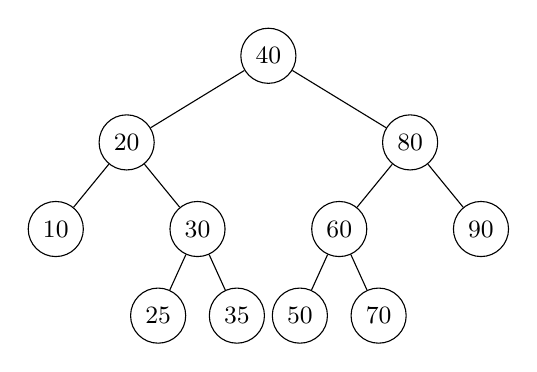
\begin{tikzpicture}[n/.style={circle,draw,inner sep=0pt,minimum size=7mm,font=\small},
  level distance=11mm, level 1/.style={sibling distance=36mm}, level 2/.style={sibling distance=18mm},
  level 3/.style={sibling distance=10mm}]
\node[n] {40}
  child {node[n] {20} child {node[n] {10}} child {node[n] {30} child {node[n] {25}} child {node[n] {35}}}}
  child {node[n] {80} child {node[n] {60} child {node[n] {50}} child {node[n] {70}}} child {node[n] {90}}};
\end{tikzpicture}
\end{center}
\begin{enumerate}[leftmargin=2.6em, labelsep=0.4em]
\item[㈠] 加入資料 27。（6 分）
\item[㈡] 加入資料 45。（6 分）
\item[㈢] 加入資料 95。（6 分）
\end{enumerate}
\end{pastexam}

\begin{pastsoln}
作法（資結書第~10.2.3~節）：先照二元搜尋樹的規則插入，再從新節點往根走，找第一個左右子樹高度差
變成 $2$ 的節點（最低的失衡節點），依新節點在它底下的方向（LL、LR、RR、RL）做一次或兩次旋轉。
以下高度以葉節點為 $1$ 計，平衡因子 $\mathit{bf} = $ 左子樹高 $-$ 右子樹高。 原樹 T 各節點的
$\mathit{bf}$：40 是 $0$（兩邊都高 $3$），20 是 $-1$，80 是 $+1$，30、60 是 $0$。

\textbf{㈠ 加入 27}。 路徑 $40 \to 20 \to 30 \to 25$，$27 > 25$，放在 25 的右子。 往上檢查：25 的
$\mathit{bf} = -1$；30 的 $\mathit{bf} = +1$（左高 $2$、右高 $1$）；20 的左子樹高 $1$、右子樹高 $3$，
$\mathit{bf} = -2$，失衡。 新節點在 20 的右子（30）的左子樹（25）裡，是 \textbf{RL} 型：先對 30 右旋，
再對 20 左旋，25 升上來當這棵子樹的根，20 和 30 分別成為它的左、右子，25 原本的右子 27 改接到
30 的左邊。
\begin{center}
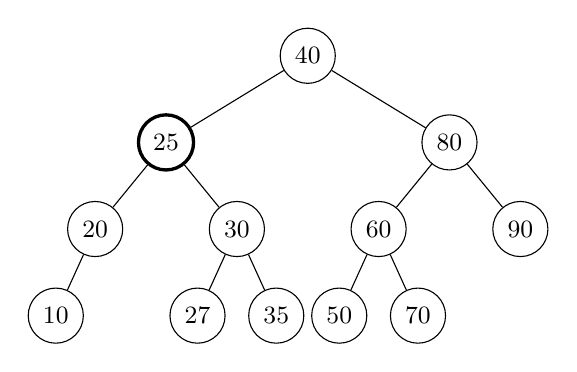
\begin{tikzpicture}[n/.style={circle,draw,inner sep=0pt,minimum size=7mm,font=\small},
  level distance=11mm, level 1/.style={sibling distance=36mm}, level 2/.style={sibling distance=18mm},
  level 3/.style={sibling distance=10mm}]
\node[n] {40}
  child {node[n,very thick] {25} child {node[n] {20} child {node[n] {10}} child[missing]} child {node[n] {30} child {node[n] {27}} child {node[n] {35}}}}
  child {node[n] {80} child {node[n] {60} child {node[n] {50}} child {node[n] {70}}} child {node[n] {90}}};
\end{tikzpicture}
\end{center}
檢查：25 的兩邊都高 $2$；20 的 $\mathit{bf} = +1$，30 的 $\mathit{bf} = 0$；40 兩邊仍都高 $3$。
中序是 10, 20, 25, 27, 30, 35, 40, 50, 60, 70, 80, 90。

\textbf{㈡ 加入 45}。 路徑 $40 \to 80 \to 60 \to 50$，$45 < 50$，放在 50 的左子。 往上：50 的
$\mathit{bf} = +1$；60 的 $\mathit{bf} = +1$（左高 $2$、右高 $1$）；80 的左子樹高 $3$、右子樹高 $1$，
$\mathit{bf} = +2$，失衡。 新節點在 80 的左子（60）的左子樹（50）裡，是 \textbf{LL} 型：對 80 右旋
一次。 60 升上來，80 成為 60 的右子，60 原本的右子 70 改接到 80 的左邊。
\begin{center}
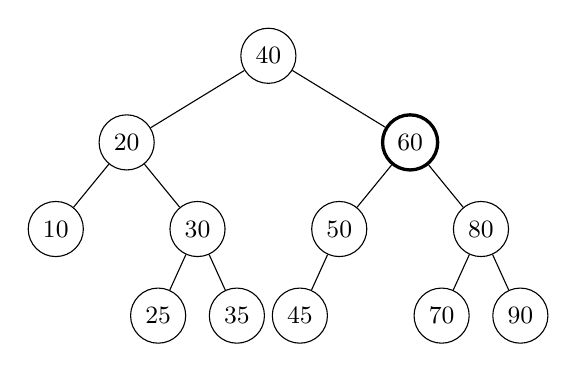
\begin{tikzpicture}[n/.style={circle,draw,inner sep=0pt,minimum size=7mm,font=\small},
  level distance=11mm, level 1/.style={sibling distance=36mm}, level 2/.style={sibling distance=18mm},
  level 3/.style={sibling distance=10mm}]
\node[n] {40}
  child {node[n] {20} child {node[n] {10}} child {node[n] {30} child {node[n] {25}} child {node[n] {35}}}}
  child {node[n,very thick] {60} child {node[n] {50} child {node[n] {45}} child[missing]} child {node[n] {80} child {node[n] {70}} child {node[n] {90}}}};
\end{tikzpicture}
\end{center}
檢查：60 兩邊都高 $2$，50 的 $\mathit{bf} = +1$，80 的 $\mathit{bf} = 0$；40 兩邊都高 $3$。

\textbf{㈢ 加入 95}。 路徑 $40 \to 80 \to 90$，$95 > 90$，放在 90 的右子。 往上：90 的
$\mathit{bf} = -1$；80 的左子樹（60）高 $2$、右子樹（90）高 $2$，$\mathit{bf}$ 由 $+1$ 變成 $0$；
80 的高度仍是 $3$，40 的 $\mathit{bf}$ 不變，是 $0$。 沒有節點失衡，不必旋轉。
\begin{center}
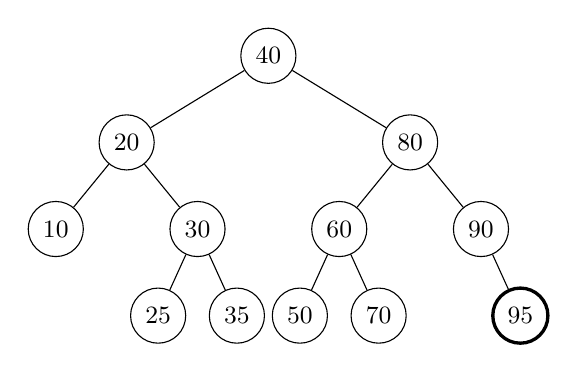
\begin{tikzpicture}[n/.style={circle,draw,inner sep=0pt,minimum size=7mm,font=\small},
  level distance=11mm, level 1/.style={sibling distance=36mm}, level 2/.style={sibling distance=18mm},
  level 3/.style={sibling distance=10mm}]
\node[n] {40}
  child {node[n] {20} child {node[n] {10}} child {node[n] {30} child {node[n] {25}} child {node[n] {35}}}}
  child {node[n] {80} child {node[n] {60} child {node[n] {50}} child {node[n] {70}}} child {node[n] {90} child[missing] child {node[n,very thick] {95}}}};
\end{tikzpicture}
\end{center}
三個小題分別是雙旋轉、單旋轉、不旋轉三種情形：插入點落在原本較矮的一側（95 加在 80 較矮的
右邊）只會讓樹更平衡；落在原本較高的一側，就要看是外側（LL、RR）還是內側（LR、RL）。
\end{pastsoln}
